\chapter{\textsc{Kiến trúc hệ thống}}
\label{chapter3}
Từ những cơ sở lý thuyết thu thập ở chương 2, chương này em sẽ trình bày những bước giải quyết bài toán mà đề tài đưa ra.
\section{Mô hình kiến trúc tổng quan}
		\begin{figure}[h!] % hinh 215
			\centering
			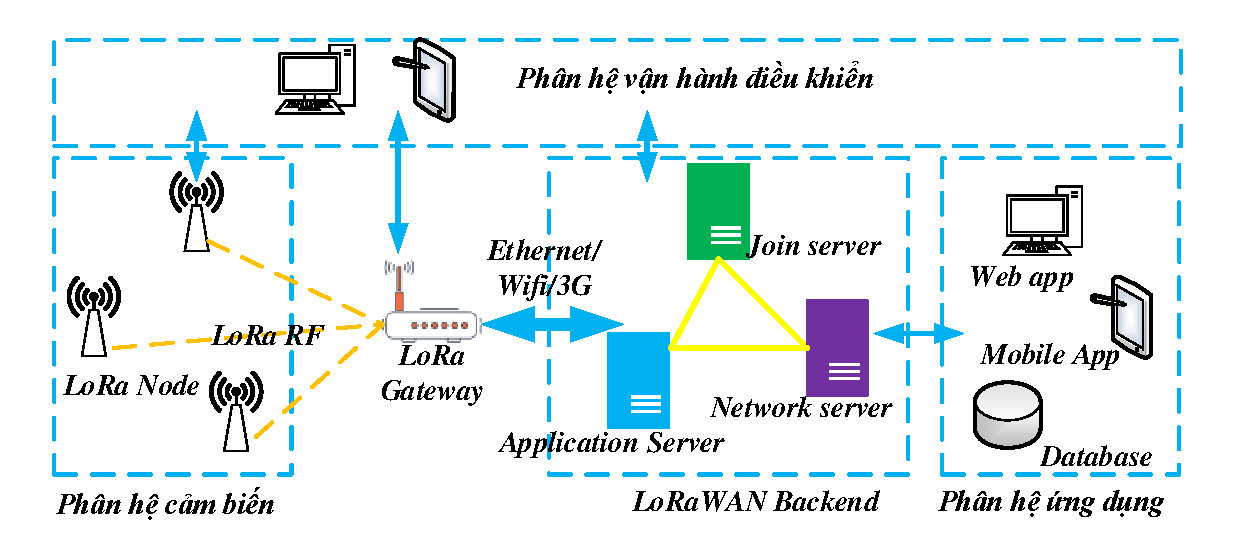
\includegraphics[width=\linewidth]{./img/31.pdf}
			\caption{Mô hình kiến trúc hệ thống}
			\label{fig:fig31}
	\end{figure}
Dựa trên các mô hình truyền thông dành cho mạng sử dụng công nghệ truyền thông cự ly lớn và công suất thấp. Cũng như tham chiếu cho mô hình kiến trúc truyền thông của chuẩn LoRaWAN Alliance, em đề xuất mô hình kiến trúc hệ thống truyền thông sử dụng LoRaWAN ứng dụng trong quan trắc các tham số môi trường, phóng xạ,.. như Hình \ref{fig:fig31}. Trong kiến trúc hệ thống đề xuất gồm các phân hệ như sau:
\begin{itemize}
\item	Phân hệ cảm biến: Phân hệ này bao gồm các thiết bị quan trắc, đo lường các tham số môi trường bằng các loại cảm biến chuyên dụng, chính xác. Các dữ liệu đo được từ cảm biến sẽ được gửi đến LoRaGateway bằng sóng LoRa RF,
\item	Phân hệ LoRaBackend: Phân hệ đề xuất thiết kế triển khai theo LoRa Backend của chuẩn LoRaWAN bao gồm Join Server, Network server và Application Server,
\item	Phân hệ ứng dụng, phân hệ này bao gồm các hệ quản trị dữ liệu lưu trữ dữ liệu đã nhận được, và triển khai các ứng dụng liên quan như website, ứng dụng mobile hoặc ứng dụng học máy (machine learning), học sâu (deep learning). (Không nằm trong phạm vi đồ án này),
\item	Phân hệ vận hành, điều khiển: Phân hệ này có chức năng giám sát, điều khiển, cấu hình thiết bị từ xa. 
\end{itemize}

\section{Phân hệ cảm biến (LoRa Nodes)}
Phân hệ cảm biến là tập hợp các thiết bị node cảm biến có các chức năng như sau:
\begin{itemize}
\item	Tích hợp các module cảm biến đo đạc các tham số vật lý môi trường tuỳ thuộc vào các ứng dụng cụ thể như: đo đạc các nồng độ phóng xạ ứng dụng trong kiểm xạ hoặc giám sát, phát hiện nguồn phóng xạ. Các loại cảm biến đo các thông số môi trường nước ảnh hưởng đến nuôi trồng thuỷ hải sản như H2S, DO, độ mặn, pH,… nhằm ứng dụng trong các ứng dụng nông nghiêp thông minh. Đơn giản hơn để kiểm tra có thể các cảm biến đơn giản như cảm biến nhiệt độ, độ ẩm, cảm biến khí gas, khói bụi ứng dụng trong các toà nhà, văn phòng, …
\item	Thiết bị nút cảm biến phải có chức năng hiệu chỉnh xử lý tín hiệu thu được từ các đầu vào cảm biến, xử lý đề đưa ra dữ liệu số trước khi truyền đi,
\item	Chức năng tiếp theo là chức năng truyền thông, với mạch LoRa node đưa ra sẽ dựng module truyền thông LoRa của Semtech triển khai chuẩn LoRaWAN là công nghệ truyền thông chính. Với chức năng truyền thông này, dữ liệu được đảm bảo bảo mật, truyền thông chính xác, hiệu quả đường truyền, hiệu quả sử dụng phổ cao. Khoảng cách thiết kế cần đạt khi truyền thông bằng module LoRaWAN yêu cầu 7-10 km với tầm nhìn thẳng. 2-3 km trong phạm vi đô thị. Ngoài ra, em cũng đề xuất tích hợp thêm module GSM, module Sim, ưu điểm của module SIM là truyền thông được xa, có hạ tầng kỹ thuật của các nhà mạng hỗ trợ cao nên có thể truyền trực tiếp dữ liệu về server. Nhưng nhược điểm lớn nhất phải kể đến là tốn kém chi phí. Vì giá thành của một module SIM dao động từ 500.000 vnđ trở lên. Trong khi module LoRa chỉ từ 200.000 – 400.000 vnđ. Hơn nữa khi gắn module sim lên thiết bị, việc bảo trì, nạp cước, đăng ký gói dịch vụ mạng cũng phức tạp, gây phiền phức cho người bảo trì khi các số lượng các node truyền thông lớn và nằm giải rác với khoảng cách lớn. Hoặc các node được lắp đặt tại những nơi khó tiếp cận như gắn trên phao đặt trong một vịnh, đầm nuôi tôm,… 
\item	Thiết bị node phải có chức năng cảnh báo, báo hiệu sự hoạt động của hệ thống bằng các đèn led hoặc hiển thị thông tin, trạng thái thiết bị ra ngoài màn hình LCD. 
\item	Chức năng định vị được đưa ra nhằm xác định vị trí của thiết bị. Việc nắm được vị trí của thiết bị nhằm khiến cho nội dung dữ liệu mà thiết bị gửi lên ứng dụng có giá trị khi được gắn với một không gian và thời gian cụ thể. Ngoài ra, việc định vị còn giúp xác định được thiết bị khi bị thất lạc hoặc có bản đồ toàn cụ sự bố trí vị trí các mạng cảm biến, nhằm có những điều chỉnh hợp lý tuỳ vào các ứng dụng cụ thể. 
\end{itemize}

\section{Phân tích yêu cầu chức năng LoRa-Gateway}
Với LoRa Gateway đề ra những chức năng cơ bản như sau (tuân theo chuẩn LoRaWAN):
\begin{itemize}
\item	LoRa Gateway có chức năng nhận dữ liệu (các bản tin dữ liệu hoặc điều khiển) được gửi từ LoRa Node thông qua phương thức điều chế LoRa. LoRa Gateway phải phục vụ được nhiều node. Theo nhà cung cấp module Semtech thì một LoRa Gateway có thể phục vụ được 10.000 nodes. Với đồ án đặt ra, em sẽ thử nghiệm với số lượng node tối đa mà làm được. Tối thiểu sẽ là 2 nodes. Cơ chế đa truy nhập sử dụng chung tài nguyên đường truyền vô tuyến LoRa giữa các LoRa Nodes và Gateway được triển khai cài đặt nhằm giảm thiểu sự va chạm và tăng hiệu suất đường truyền,
\item	LoRa Gateway chuyển tiếp bản tin uplink về LoRa Backend và chuyển tiếp bản tin downlink xuống các LoRa Node. Kết nối giữa LoRa Gateway và LoRa Backend được phân tích, thiết kế, triển khai sẽ sử dụng chuẩn IEEE 802.3, IEEE 802.11 và sử dụng module SIM 3G (tuỳ chọn).
\end{itemize}
\section{Phân tích yêu cầu chức năng phân hệ LoRa Backend }
	\begin{figure}[h!] % hinh 32
			\centering
			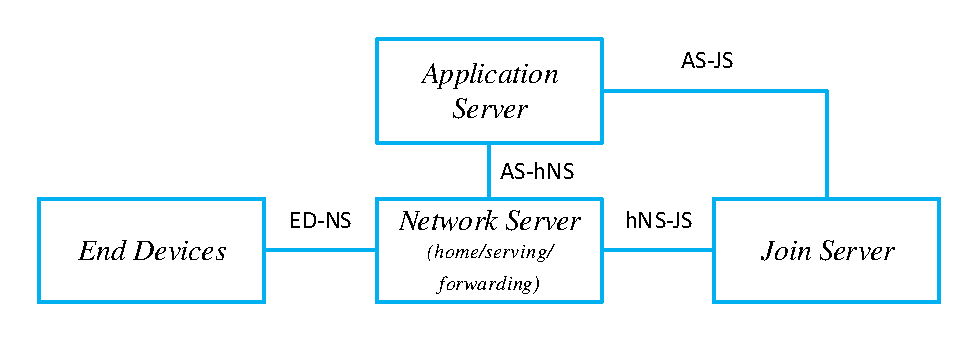
\includegraphics[width=\linewidth]{./img/32.pdf}
			\caption{Mô hình tham chiếu LoRa Backend với các thiết bị LoRa Node tại mạng nhà mình (End Device At Home) [8]}
			\label{fig:fig32}
	\end{figure}
Tham khảo dựa theo đặc tả trong chuẩn LoRaWAN cụ thể trong đặc tả LoRaWAN Backend Interface (giao diện backend của mạng LoRaWAN), Hình \ref{fig:fig32} minh hoạ sơ đồ tham chiếu các phần tử của LoRaWAN Backend. Em cũng đưa ra những chức năng cơ bản phân hệ backend dành cho LoRaWAN.

\subsection{Network Server}
Network server (máy chủ quản lý mạng): là điểm của của tầng LoRa MAC phục vụ các node kết nối với mạng. Nó là trung tâm của topology hình sao mà chuẩn LoRaWAN đề ra, NS gồm các chức năng sau đây:
\begin{itemize}
\item	Kiểm tra địa chỉ các LoRa Nodes,
\item	Xác thực khung (Frame Authentication) và kiểm tra đếm khung,
\item	Phản hồi ack,
\item	Thực hiện chức năng đáp ứng data rate,
\item	Đáp ứng, phản hồi tất cả các câu lệnh yêu cầu từ lora node,
\item	Chuyển tiếp dữ liệu uplink đến đúng server ứng dụng cụ thể,
\item	Vận chuyển, queuing bản tin downlink từ server ứng dụng xuống các lora node,
\item	Vận chuyển bản tin Join-Request và Join-Accept giữa lora node và Join-server trong quá trình kích hoạt thiết bị từ xa (OTAA).
\end{itemize}
Có thể tách NS ra thành 3 phần tử gồm: (i) Serving Server (sNS); (ii) Home Server (hNS); và (iii) forwarding server (fNS). Mỗi phần tử có một chức năng cụ thể. Tuỳ vào, mô hình tham chiếu Device At Home hoặc Roaming mà 3 phần từ này được triển khai cùng một server hoặc khác các server vật lý. Chức năng cụ thể cùng từ phần tử như sau:
\begin{itemize}
\item	Serving Server: Điều khiển MAC Layer,
\item	Home Server: Là nơi lưu trữ các thông tin như sau: thông tin thiết bị, thông tin về dịch vụ, thông tin định tuyến, và DevEUI của thiết bị. hNS kết nối trực tiếp với jNS nhằm phục vụ quá trình kích hoạt, đăng ký tham gia vào mạng của lora nodes. hNS cũng kết nối trực tiếp với AS nhằm vận chuyển các bản tin uplink và downlink giữa hai phần từ. 
\item	Forwarding server: là phần tử quản lý kết nối với Radio Gateway, nó quản lý các bản tin uplink, downlink giữa GW và sNS.
\end{itemize}

\subsection{Join Server}
JS quản lý quá trình OTAA, JS sẽ sử dụng các thông tin sau để thực hiện quá trình điều khiển:
\begin{itemize}
\item	DevEUI,
\item	AppKey,
\item	NwkKey (chỉ sử dụng với LoRaWAN v1.1 Device),
\item	Bộ định danh Home Network Server,
\item	Bộ định danh máy chủ ứng dụng,
\item	Phiên bản LoRaWAN (1.0, 1.0.2, 1.0.3 hoặc 1.1) 
\end{itemize}
\subsection{Application Server }
Server ứng dụng (Application Server) xử lý các payload của tầng ứng dụng, cung cấp các dịch vụ mức ứng dụng cho người dùng. Nó cùng sinh ra các bản tin downlink gửi xuống các thiết bị lora node.

\section{Phân tích chức năng phân hệ ứng dụng người dùng}
Phân hệ chức năng ứng dụng người dùng, khai thác các dữ liệu thu thập được từ các LoRa Nodes gửi lên xử lý và thao tác với chúng tuỳ từng ứng dụng cụ thể. (Phân hệ này không bao gồm trong đồ án này)

\section{Phân tích chức năng phân hệ vận hành điều khiển}
Những chức năng đặt ra ở phân hệ này gồm:
\begin{itemize}
\item	Có khả năng thực hiện vận hành, điều khiển, kiểm soát lỗi, kiểm tra tình trạng thiết bị bằng cách kết nối trực tiếp thiết bị lora node, gateway với các thiết bị điều khiển như PC, …
\item	Có khả năng cấu hình, yêu cầu trạng thái và điều khiển một số tác vụ quan trọng từ xa bằng các phương pháp cấu hình qua tin nhắn hoặc qua các câu lệnh điều khiển qua Internet thông qua hệ thống. 
\end{itemize}

\section{Kết luận}
Trong chương này, dựa trên những kiến thức về cơ sở lý thuyết LoRa, LoRaWAN cũng như các phần kiến thức về thiết kế hệ thống truyền thông. Em đã đưa ra mô hình kiến trúc mạng truyền thông tổng quan sử dụng công nghệ truyền thông LoRa, áp dụng theo mô hình chuẩn LoRaWAN Alliance. Cụ thể hơn, em cũng nêu ra những chức năng chính của từng phân hệ - phần tử của hệ thống. Trong các chương tiếp theo em sẽ trình bày chi tiết các giải pháp kỹ thuật, thiết kế, lựa chọn linh kiện phần cứng, và đưa ra những lưu đồ thuật toán, cấu trúc firmware nhằm điều khiển, cài đặt tại từng phân hệ khác nhau.   